%
% 1
%
\chapter{Introduction}%
	%
	\label{ch:intro}
	\index{Course!Introduction}%
	%
  \begin{mybox}%
    %
    \newthought{Dear reader,}\\[1em]%
  	%
  	You probably find yourself reading this because you enrolled in Statistical Reasoning and Quantitative Methods (\SRQM), a postgraduate introduction to statistics that Ivaylo Petev and myself have been teaching at Sciences~Po in Paris since 2010.\\[1em]%
    %
    Welcome to the course.\\[1em]%
    %
    \smallcaps{This guide} is a practical handbook to read while taking the course. The rest of the teaching material, which includes the syllabus and essential files to be used in and outside class, can be downloaded from the course webpage at the following address:\\[1em]%
      %
      \url{http://www.joelgombin.fr/teaching/quanti/}\\[1em]%
      %
  	%
    \smallcaps{Start reading below} to learn about the course basics, making sure in particular that you have \textbf{run the course setup} on your computer and that you know how to run it again if necessary. Welcome again, and see you soon.%
    %  
  \end{mybox}\\[4em]%
  %
  \startcontents[chapters]%
  \printcontents[chapters]{l}{1}{\setcounter{tocdepth}{2}}%
	%
	\newpage%
	%

%
% 1.1 course topics
%
%
% 1.1
%
\section{Course essentials}%
	%
	%
	\label{sec:topic}%
	\index{Methods}%
	%
	%

	\newthought{The approach to social science} that we follow in this course is driven by a dual logic of inquiry: we start with the description of quantitative data, and we end with its analysis through statistical models. The procedures involved in this process are computational and require some technical knowledge of computers and mathematics.%
		%
		%

		%%% They’re someone who can ask and answer questions about and with data.
		%%% http://www.analyticstory.com/hadley-wickham/

		%%% I A key principle in applied statistics is that you should be able to connect between the raw data, your model, your methods, and your conclusions

		%%%%Controlled experiments are the gold standard, but I never do them!

	%%% I (Some) computer scientists' view: we don't need controlled experiments; we can automatically learn from observational data

	%%% I Psychologists' view: each causal question requires its own experiment

	%%% I Observational scientist's version: each causal question requires its own data analysis
	
	%%% Sample surveys (for the problem of extending from sample to population)

	%%% Descriptive observational research (for the problem of modeling complex interactions and response surfaces)

	%%%Political science is largely an empirical discipline. That is, most of us studying politics do so because we are motivated by real world political events, either historical, current, or even events yet to happen. We want to know why these events happen and how to make sense of them. Political science trys to answer these questions in a rigorous way. Data analysis is thus a critical component of political science, serving two important purposes: (1) providing numerical descriptions or summaries of political phenomena, facilitating comparisons across time, countries, states, people, etc; (2) testing theories, models and hypothesis about politics.


% All this is to say that this class involves a little math. Or, as I like to put it, this class is ‘‘techie for fuzzies’’: an introduction to the way political scientists use the tools of statistics to rigorously understand political events. I assume virtually zero mathematical background on your part, either because you didn’t take math in high school or because you’ve forgotten it. I assume no prior background with using computers for data analysis. The classes will have a heavy ‘‘show-and-tell’’ feel to them, where I will use statistical software to do data analysis.

	%%%forecast the effects of interventions, the trajectory of existing trends, and the likely strategies
	
	%%% http://understandingsociety.blogspot.fr/2009/01/predictions.html
	
	% 1.1.1
	%
	\subsection{Quantitative methods}%
		%
		\label{sec:quantitative-methods}
		\index{Quantitative methods}%
		%
		%

	\newthought{Quantitative methods} designate a branch of social science methodology that applies statistical procedures to experimental or observational data in order to produce explanatory models for the complex, recurrent phenomena that affect populations and organizations. These methods can be used to analyze things like attitudes towards highly skilled and low-skilled immigration in the United States,\footcite{HainmuellerHiscox:2010a} the effects of a program to develop fertilizer use in Kenya,\footcite{DufloKremer:2009a} or the historical vote that put Adolf Hitler into power in interwar Germany.\footcite{KingRosen:2008a}%
		%
		%

	The models produced by quantitative research account for the regularities that exist in the data by estimating how a set of independent, explanatory variables can predict the value of a dependent, outcome variable. To what extent, for example, is the prevalence of HIV/AIDS predictable from the level of economic inequality and degree of political unrest in a country? Does the support for violent action vary with age and education, in what direction, by how much, within what range and at what rate? A quantitative model can estimate these relationships, on top of which researchers develop theories to explain what causal paths are followed in the model.%
		%
		%

	A strong background assumption behind such questions is comparability. In quantitative data, the units of observation, such as individuals or countries, are defined through a set of commensurable characteristics—the variables. The first and perhaps most important requirement of a quantitative model is that you are measuring roughly the same thing among roughly similar units with sufficient reliability. This is far from obvious when you are aggregating, for instance, development statistics, because many countries have very low statistical capacity (among many other issues).\footcite{Jerven:2013a}%
		%
		%

	Each variable of a quantitative model is then attached to a concept, like `household income' or `democratic status,' each of which provides an explanatory component for the dependent variable. Measuring the predictive effect of the `independent' variables onto the `dependent' one is therefore a means to measure the respective influence of each explanatory component onto a given phenomenon, which might be a measure of something, like the number of children in a household or the GDP growth rate of a country, or the probability of occurence of something, like abortion or state collapse.%
		%
		%

	\newthought{From a learning perspective,} what you can immediately figure out of the short description above is that quantitative methods require some attention to terminology: `data' are `observations' described by `variables' made of `values', some of which we `predict' from the others through the `estimation' of their `independent' effects. The topic also requires some (really light) exposure to logic and mathematics. Finally, any quantitative analysis requires some knowledge of the practical aspects of empirical research design, such as data collection or sampling.%
		%
		%

	Contrary to what bookshelves of statistics textbooks and horror stories about equations feeding on human flesh might have led you to believe, your learning approach of quantitative analysis should actually have much more to do with its practice than with its theory. The practice of quantitative data analysis implies, for example, that you have to try things out until `they work' at the technical level. This aspect of things requires a lot of independent learning through trial-and-error.%
		%
		%
	
	Another practical dimension of quantitative analysis in the social sciences has to do with the limited degree of precision of any social statistic, which makes issues of statistical significance secondary to issues of measurement accuracy and data availability when it comes to social data. When your unit of analysis is a social one, start thinking in rounded figures: the measures are never more precise than what they are, nor the data more representative than what it can possibly be.%
		%
		\footnote{For that matter, a report that would speak of `1.474\% of the general population' is almost never going to be a credible result with social data, because three-digit precision would indicate spectacularly precise estimation.}%
		%
		%
		
% 1.1.2
%
\subsection{Course outline}%
	\index{Course!Outline}

\newthought{The course} is organised in twelve two-hour sessions that run over a single semester. Its content is structured around three teaching goals:%

\begin{enumerate}
  
  % 1. Statistics

	\label{sec:textbooks}%
	\index{Course!Readings}%
  \item The course covers some \textbf{essential aspects of statistical analysis}, from describing variables to running regression models. %
 	  %
  	This learning objective requires that you read from textbooks that apply fundamental statistical theory to social science research. The primary handbook for this course is \citetitle{Urdan:2010a}\footcite{Urdan:2010a}, one of the shortest and most effective introduction to the course topics. %
	
		Towards the end of the class, we turn to \citetitle{FeinsteinThomas:2002d}\footcite{FeinsteinThomas:2002d}, a clearly worded introduction to quantitative methods for qualitatively-minded social scientists, for additional clarifications on regression modelling.%
  
		\index{Course!Syllabus}%
  	Both textbooks appear in the course syllabus%
		\footnote{\url{https://github.com/briatte/srqm/blob/master/course/syllabus.pdf?raw=true}} as well as in the final bibliography of this document. Please read the course syllabus in full at that stage, and copy the reading schedule to your agenda.%
		
		Note that the course slides will definitely \emph{not} contain enough material for you to understand the theoretical underpinnings of the methods used in class, and that if you skip the readings, it will inevitably reflect on the general quality of your analysis.%

  % 2. Stata

  \item The course also explains \textbf{how to operate Stata}, a statistical software produced by StataCorp. %
	  %
	  StataCorp is a U.S. company that also publishes journal articles and handbooks to assist users in using their software.%
		%
		\footnote{\url{http://stata.com/}} %
		%
		Some Stata Press handbooks, like the recent one by \citeauthor{Mitchell:2012a} on applied regression, can be used as companions to this course.%
		%
		\footnote{See an indicative list of references at % 	
			\url{https://github.com/briatte/srqm/wiki/stata}} %
		
		Learning to use Stata requires using a computer for research, not just as a clever typewriter or as a Web terminal; it requires practice with using keyboard shortcuts and managing files. The next pages will explain what specific computer skills you will be working on during the course.%
		
		The baseline advice to survive the computing component of the course is very simple: practice by writing code every week of class. If this is going to be the only time in your student life where you get to write statistical code, make sure that you get the most out of it. There is a fair chance that you will be offered to use that skill one day.%

  % 3. Research

  \item The course finally works assists students to work in pairs over \textbf{small-scale research projects}, on which the grading for the course is based. %
	  %
		The course was conceived with a hands-on focus and is organised around the  writing of an empirical research paper supported by a replication script written in Stata code. Each student pair submits two draft versions of the code and paper during the semester, and one final version at the end of the class.%
		%
		%
		
		As indicated in the course syllabus, you can turn to \citeauthor{BoothWilliams:2003v}'s \citetitle{BoothWilliams:2003v}\footcite{BoothWilliams:2003v} for a detailed explanation on how to prepare a research project if you have no experience in social research, and to \citeauthor{White:2005a}'s \citetitle{White:2005a}\footcite{White:2005a} if you need a refresher on how to write an empirical research paper. All other instructions about the project are covered exclusively in class, which you should attend every week and catch up if absent.%
		%
		\footnote{The course sessions are cumulative: you cannot just skip one as if it had never happened. Your weekly workload \emph{will} extend considerably if you skip one week with the hope of catching up later or at the last minute–both strategies that \emph{never} play out well.}%
		%
		%
		
		You are encouraged to use your research project for other purposes than this course: think of it as work that you will be able to add to your student portfolio.%
		%
		%

\end{enumerate}

	\index{Course!Computer requirements}%
	The course requires that you have access to a recent computer that can connect to the Internet, read/write \PDF files and uncompress \ZIP archives, all of which are native features on most current systems. The course also requires that you can use Google Documents to edit, share and backup your research project files.%
	\footnote{\url{https://docs.google.com/}}%
	%
	%

  If you have never used a computer before to carry empirical work with statistical software, or if your self-assessed level of familiarity with computers is dramatically low, then it would be a good idea to also cover Appendix~\ref{ch:computers}, which introduces computer hardware, software and programming.%
  \footnote{Besides building up your computer skills, there are extrinsic reasons to why you should be paying some attention to computing in the current times; see Cory Doctorow, ``The Coming War on General Computation'', 2011: \url{https://github.com/jwise/28c3-doctorow/blob/master/transcript.md}}%
  %
  %

% 1.1.3
%
\subsection{About this guide}%
	%
	%
	\newthought{This `Stata guide'} was written as an introduction to Stata for students with a background in the social sciences. You are not expected to know anything about statistics, but you are expected to know a few things about social science research from your undergraduate curriculum. You should be familiar, for instance, with notions like cultural capital, gross domestic product per capita and political regimes.%
		%
		%

	We will cover the following topics:%

	\begin{itemize}
		\item This introduction deals with the course basics, essential computer skills and Stata fundamentals. It also explains how to set up a computer for the course.%
	
		\item %
		Section~\ref{ch:data} explains how to prepare data for analysis, and %
		Section~\ref{ch:distr} explains how to visualize distributions. This segment is primarily about description and univariate statistics. %
    It ends on instructions to submit your first draft.
	
		\item %
		Section~\ref{ch:asso} introduces statistical significance tests, and %
		Section~\ref{ch:ols} introduces ordinary least squares and simple linear regression. This segment is about association and bivariate statistics. %
    It ends on instructions to submit your revised draft.

		\item %
		Section~\ref{ch:lin} introduces multiple linear regression modelling, and %
		Section~\ref{ch:log} introduces logistic regression modelling. This segment covers the basics of statistical modelling for continuous and categorical variables in cross-sectional data. %

		\item %
		Section~\ref{ch:paper} contains the instructions to submit the final paper, and the appendix add some detail about the course material and requirements.%
    
    The guide also includes an index including all commands cited in the text, and a list of bibliographic references.%
	\end{itemize}

\newthought{Several sections of the guide are still in draft form}, so watch for updates and read it along other documentation. Its writing started with students questions, and several sections were first written as short tutorials concerning specific issues with data management. One thing led to another, and we ended up with the current document. The aim is to cover 90\% of the course by version 1.0.%

	Several students have already provided very valuable feedback on the text—thanks, and keep the feedback flowing in!%
%
%
% 1.2 using stata
%
%
% 1.3
%
\section{Using Stata}%
	%
	%
	\label{sec:stata}%
	\index{Stata!Introduction}%
	%
	%
	
	\newthought{This course uses Stata} as its statistical software of choice. Stata is used by many social scientists working with quantitative data in areas such as economics and political science.%
	%
 	\footnote{For example, you will find Stata output in some of Nate Silver's work at the \emph{New York Times} on his `FiveThirtyEight' electoral blog; see, e.g., ``'\href{http://fivethirtyeight.blogs.nytimes.com/2012/03/12/polling-in-deep-south-has-posed-challenges/}{Polling in Deep South Has Posed Challenges},'' 12 March 2012.} %
	%
	Most statistical procedures used in these disciplines know some form of implementation in Stata, and the software is supported by a large user community that meets on the Statalist mailing-list and develops packages available through the Statistical Software Components (\SSC) server at Boston University. Overall, it is a solution that provides a good middle ground between a spreadsheet editor and a statistical programming environment. The next sections explain what that means and how Stata works.%

\newthought{The next sections} are based on commands and keyboard shortcuts that appear in Stata~12 for Mac~OS~X (Mac) and Windows (Win).%
		%
		\footnote{Compatible operating systems are listed at %
		\url{http://www.stata.com/products/compatible-operating-systems/}. %
		%
		We use the `Standard Edition' (\textsc{se}) of Stata that works on most current hardware.} %
		%
		Both systems run Stata almost similarly, with only a few notable differences:% 
		
	\begin{description}

		\item[\smallcaps{On Mac~OS~X}] %
		%
		The entire Stata application folder should be located in the \texttt{Applications} folder, and you should drag the Stata application icon to your Dock for quicker access. The \texttt{Cmd} (Command) key used in keyboard shortcuts is the `Apple' key located left and right of the spacebar.%

		\item[\smallcaps{On Windows}] %
		%
		The entire Stata application folder should be located in the \texttt{Program Files} folder, or whatever your version of Windows call it, and you should drag the Stata application icon to your Taskbar for quicker access. You might use either the 32-bit or 64-bit version of the software.%

	\end{description}

	The course should run fine on older versions of Stata, given very minor adjustments to the code. The course setup has been tested on Sciences Po workstations equipped with Stata~11, for which it automatically adjusts memory and circumvents admin restrictions to install packages.%
  \footnote{Known issues and fixes are documented at %
		\url{https://github.com/briatte/srqm/wiki/troubleshooting}}%
		
		
% 0.3.1
%
\subsection{Learning statistical software}%
	%
	%
	\newthought{You have probably never used Stata}, but you probably have some limited experience with number-crunching. For most users, this happens in a numerically inaccurate environment called a spreadsheet editor, in which you can freely delete or edit the data without letting others know. In that kind of environment, programming means writing functions into cells and then hoping for the cells to stay where they are, which they never do (Figure~\ref{fig:dilbert-spreadsheets}).%
		%
		\footnote{Read some horror stories compiled by the European Spreadsheet %
		Risks Interest Group (EuSpRIG): %
		\url{http://www.eusprig.org/horror-stories.htm}} %
		%
		A vast majority of jobs done in spreadsheet environments will not even explore that territory and will instead safely focus on showing unreadable `3D' pie charts with no meaningful third dimension.%
		%
		%

		\begin{figure}
			
\includegraphics{dilbert-excel}
		  \caption{\href{http://dilbert.com/strips/comic/2007-08-08/}{Dilbert on spreadsheets}, by Scott Adams.}%
		  \label{fig:dilbert-spreadsheets}%
		\end{figure}

	Your use of Stata in this course will remind you of a few things that you might have already learnt from using spreadsheet software. This will include using keyboard shortcuts a lot to move around the interface and to do things quicker, especially with respect to text manipulation. It will also include using filters and operators like \texttt{IF} or \texttt{MEAN} that you might know from functional programming in spreadsheets.%
		%
		%
	
	Statistical programming, on the other end, is probably new to you. Its general principle works more or less like writing music for a single musician: you have to compose a sequence of instructions that enables anyone to play your stuff. The current de facto standard in statistical programming is R, a free and open source software with excellent graphics support that lets you crunch numbers like a statistician would want you to: neatly, if at the cost of intuitiveness.%
		%
		\footnote{For example, in R, the number `2' is not just a number (i.e. a scalar), it is a vector of length 1 of numeric class.} %
		%
	 	R users know that its sheer complexity and subtle idiosyncracies create a steeper learning curve for new users, and that there is ``something not fully healthy''%
		\footnote{%
			\url{https://stat.ethz.ch/pipermail/r-help/2007-August/139047.html}} %
			about it. Still, if you ever plan to enhance your statistical programming skills, R and a few other languages will become your weapon of choice. Ivaylo and myself also teach an exploratory course in R if you want to get a feel of it.%
		\footnote{\url{http://f.briatte.org/teaching/ida/}}%
	%
	%

	\newthought{Stata is a compromise} between these two worlds that lets you work on a single spreadsheet of data through a set of predefined and user-contributed commands. It compares well to the competition: its emphasis on programming is more pronounced than what it is in SPSS, which is mostly used through point-and-click, and its language is more convenient than the one used by SAS, an expensive and historically dominant statistical software that remains the only solution capable of dealing with very large datasets. Stata is also less focused on a single approach to quantitative analysis than, say, Epi Info for epidemiology or gretl for econometrics.%
		%
		%
		
	Stata has its own limitations. Its graphics engine is not bad, but it is far from excellent: the graph syntax is tiresome, and it takes lines and lines of code to escape the default plots to produce better visualizations. Despite being rather open to user-contributed commands, Stata is a commercial product with a price tag and a closed proprietary format that requires conversion to import outside of Stata. Finally, and although that can be seen as a feature of the software, Stata can only work on a single dataset at a time, because it works like an accountant's book, one page after the other.%
		%
		%

% 0.3.2.
%
\index{Computers!Graphical User Interface (GUI)}%
\index{Computers!Command Line Interface (CLI)}%
\index{Stata!Command line interface}%
%
\subsection{Working from the command line} %
	%
	% graphical user interface
	% command line
	% example: sysuse lifeexp
	%
	Stata can be used either through its Graphical User Interface (GUI), like most of the software that you use, or through a Command Line Interface (CLI), which presents itself as a terminal where the user types instructions to produce certain results. The latter approach is the programmer's way of doing things: it is much more versatile and forces you to write up your operations in the form of a script, which Stata calls a `do-file'. This file is a plain text file containing Stata code that, like a music sheet, makes it possible to understand and reproduce your analysis of the original data.%
	
	We are going to explore Stata from the command line, which relies only on three windows: the Command line window, the Results window attached to it, and the do-files window. This minimal setup is shown below in Figure~\ref{fig:stata-ide}. We will not use any other element of the graphic user interface in this course, but feel free to explore Stata and learn about its other functionalities.%
	
	\begin{figure}
		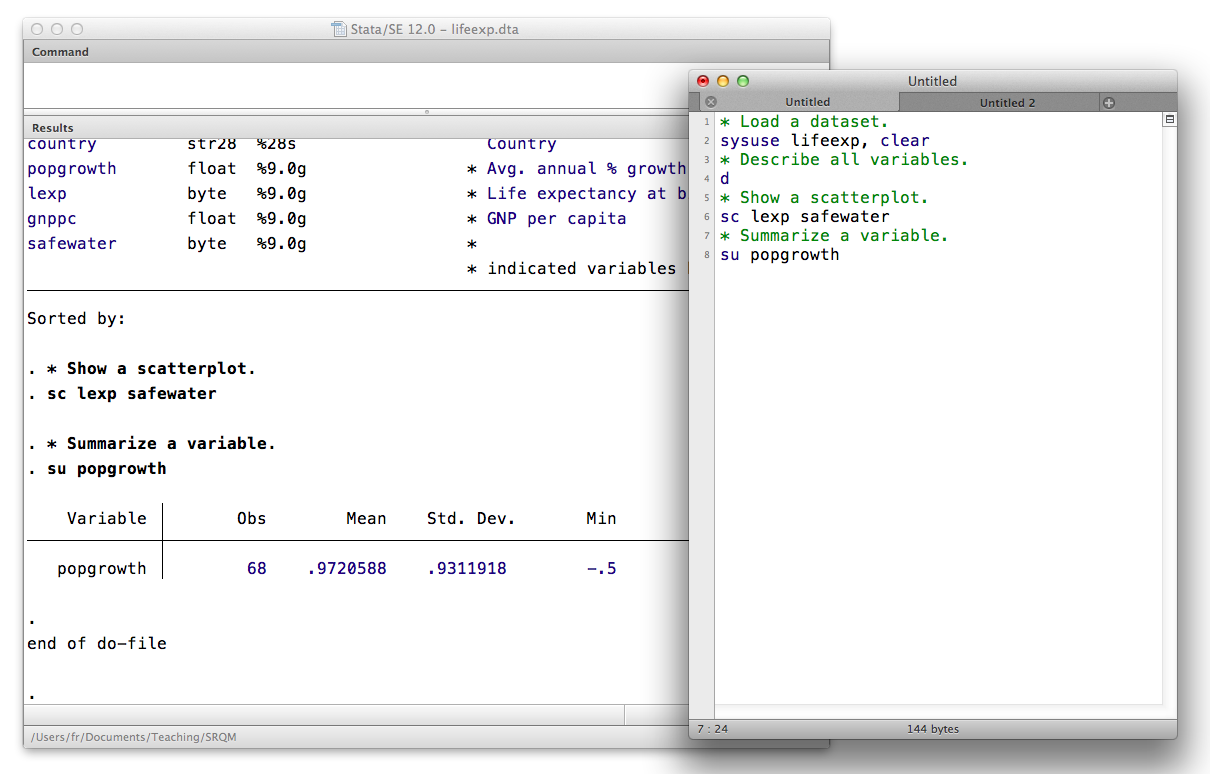
\includegraphics{stata-ide}%
		\caption{The Holy Trinity of Stata programming: the Command window (on top), the Results window (below it), and a do-file editor (in the background).}%
		\label{fig:stata-ide}%
	\end{figure}

%% -- command line

% The Stata GUI can be used occasionally for routine operations that need not appear in your do-files. Keyboard shortcuts also save some time, as with ‘File > Open…’ (Ctrl-O in Stata for Windows) or ‘File > Change Working Directory…’ (Cmmd-Shift-J in Stata for Macintosh; this document uses ‘Cmmd’ to designate the ‘’, a. k. a. ‘Command’, ‘Cmd’ or ‘Apple’ modifier key).

	The next sections explain how to run commands in Stata, and how to organize them into a do-file. A list of all commands used in the guide appear in the index, and a list of all commands used in the course appear on the course wiki.%
		\footnote{\url{https://github.com/briatte/srqm/wiki/synopsis}}%

		\begin{description}
			\item[\smallcaps{Running commands}]%
			\vspace{1em}%
			%
			In Stata, focus on the Command window by clicking into it or by pressing \texttt{Cmd-1} (Mac) or\texttt{Ctrl-1} (Win). Type the following command and press \texttt{Enter} to run the command, which means to execute its code:%
			
		\begin{docspec}%
			\label{lifeexp}%
			sysuse lifeexp, clear
		\end{docspec}
			
		If your command ran successfully, Stata will display its result:\\[1em]
			
			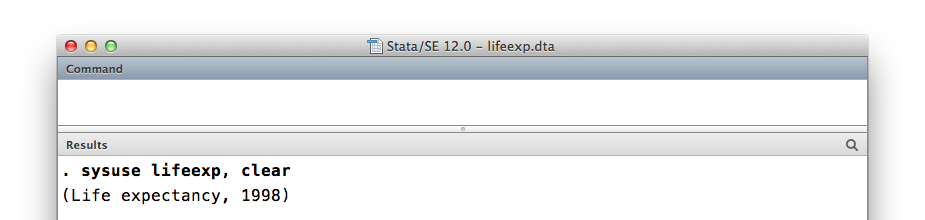
\includegraphics{stata-lifeexp-sysuse}\\[1em]

		Note that some commands produce `blank' output, which means that a command can be successfully entered and executed without printing any result. In this case, a simple \texttt{.} line dot will appear in the Results window, as to show that Stata encountered no problem while executing the command, and that it is ready to process another one.%
			%

			\item[\smallcaps{Fixing typos}] %
				\index{Stata!Syntax}%
			%
		Stata commands follow a strict syntax, and if you make a typo in a command, the software will return an error in red ink. In that case, you have to fix the issue by re-typing the command correctly. Try for example, to enter the following command:%
				%
				\marginnote{Examples with the \texttt{lifeexp} dataset %
					continued from p.~\pageref{lifeexp}.}%
			
			\begin{docspec}
				summarizze popgrowth
			\end{docspec}
			
			The mistake is rather obvious here: the \cmd[su]{summarize} command should take only one `z':\\[1em]%
			
			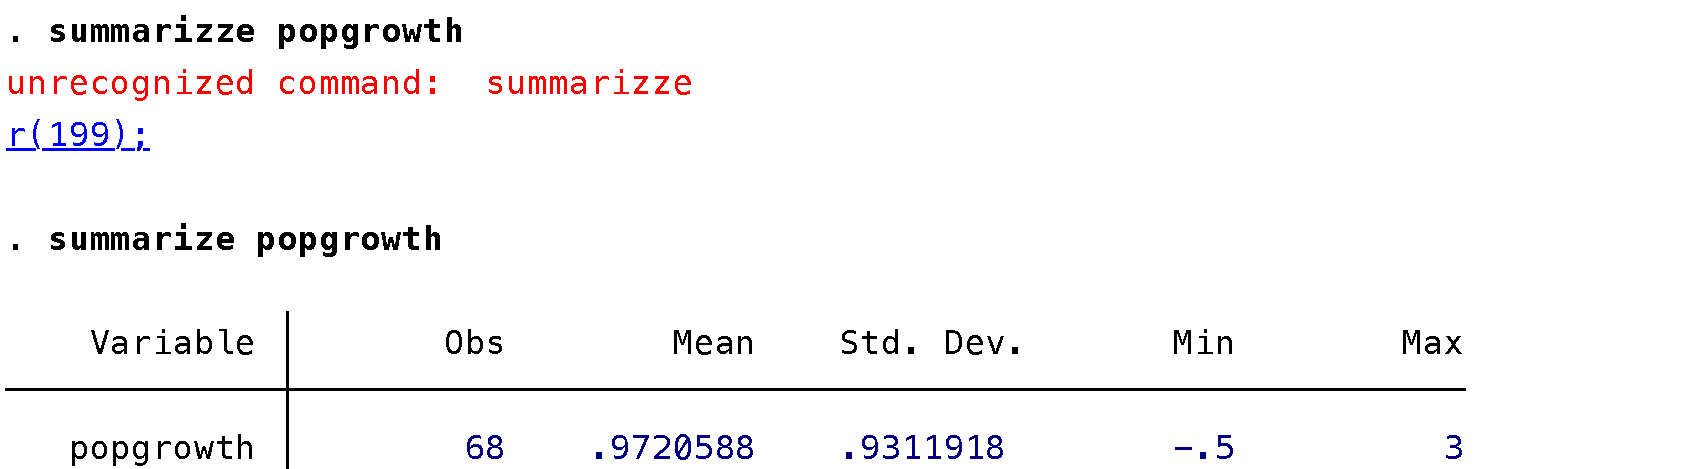
\includegraphics{lifeexp-sum-error-zz}\\[1em]
			
			If you need, as in this example, to correct a mispelled command, or to re-run a command that you have used earlier on, you should \textbf{press \texttt{PageUp} on your keyboard} to recall the previous command that you typed.%
			%
			\footnote{On laptop keyboards, \texttt{PageUp} is usually replaced by \texttt{Fn-UpArrow}. Past commands can also be examined in the Review window.} %
			%
			This allows you to fix your mistake by pulling the last command very quickly and correct only the typo, rather than having to type it again.%

			Here's another common mistake. Try the following in Stata:%
			
			\begin{docspec}
				Summarize popgrowth
				summarize POPGROWTH
			\end{docspec}

			In response to these commands, you will get more or less informative error messages. The issue here is that Stata commands are case-sensitive: the capitalized \texttt{Summarize} command is different from \texttt{summarize} command in lowercase. By that virtue, there is no variable called \texttt{POPGROWTH} in uppercase in the \texttt{lifeexp} dataset, but there is one called \texttt{popgrowth} in lowercase:\\[1em]%

			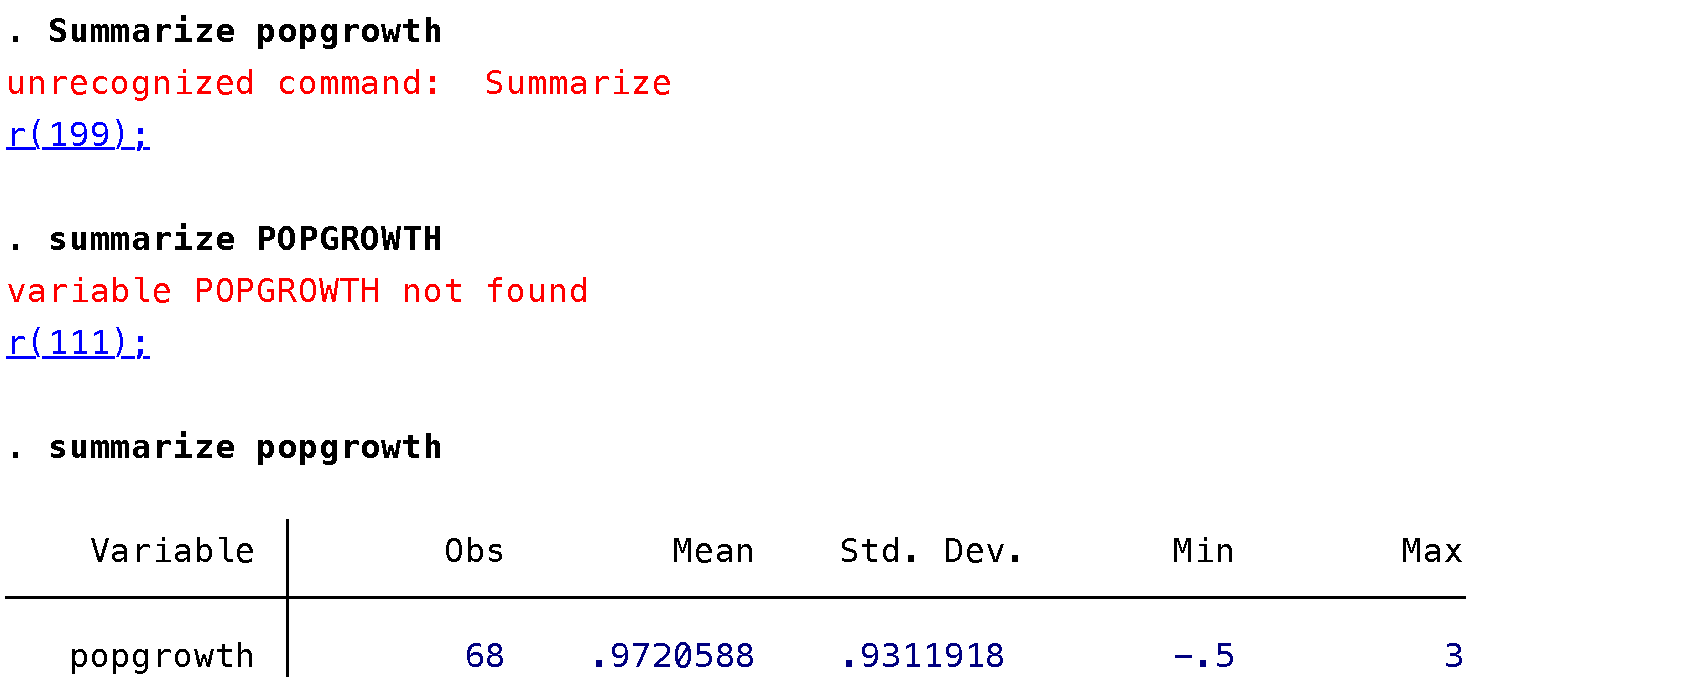
\includegraphics{lifeexp-sum-error-caps}\\[1em]
			
			Stata is usually operated in lowercase, although some variable names might show up in uppercase in some datasets. In order to keep things as straightforward as possible, avoid using uppercase yourself when naming variables.%
			
			%
			%
			\item[\smallcaps{Using help files}]%
				\index{Stata!Help files}
			%
			If you cannot find the right syntax or option for a command, turn to the technical documentation for precisions and examples of any given command. Use the \cmd[h]{help} command to access it in Stata, as in these examples:%
	
			\begin{docspec}
				* Help for the -summarize- command.\\
				help summarize\\[1em]
		
				* Help for the -lookfor- command.\\
				help lookfor
			\end{docspec}

			Stata help is also available online.%
				\footnote{\url{http://www.stata.com/help.cgi?help}} %
				
			\newthought{If you need further technical help} with Stata, refer to the course website for a selection of tutorials.%
				%
				\footnote{\url{http://f.briatte.org/teaching/quanti/}} %
				%
				A Web search with your question keywords might also work if someone has asked a similar question on Statalist or on StackOverflow.%
				%
				\footnote{\url{http://stackoverflow.com/}}%
				% 
				%

				\item[\smallcaps{Abbreviations}]%
					\index{Stata!Syntax}%
				%
				Most Stata commands can be abbreviated for quicker use. If you run the \texttt{help summarize} command, the help window will tell you that the \texttt{\underline{su}mmarize} command can be abbreviated to \texttt{su}. Type the following example in Stata to see how the language abbreviates:%
				%
				\marginnote{Examples with the \texttt{lifeexp} dataset %
					continued from p.~\pageref{lifeexp}.}%

		\begin{docspec}
			* With a command:\\%
			summarize popgrowth\\%
			su popgrowth\\[1em]%
			%
			* With help pages:\\%
			help summarize\\%
			h su%
		\end{docspec}

	Note that the bottom lines show you how to open help pages with the single letter \texttt{h}, which is handy when you are often brought to verify syntax and read examples from the documentation. This guide shows commands that can be abbreviated in both forms, as with \cmd[su]{summarize}, which is shown in the example:\\[1em]%

		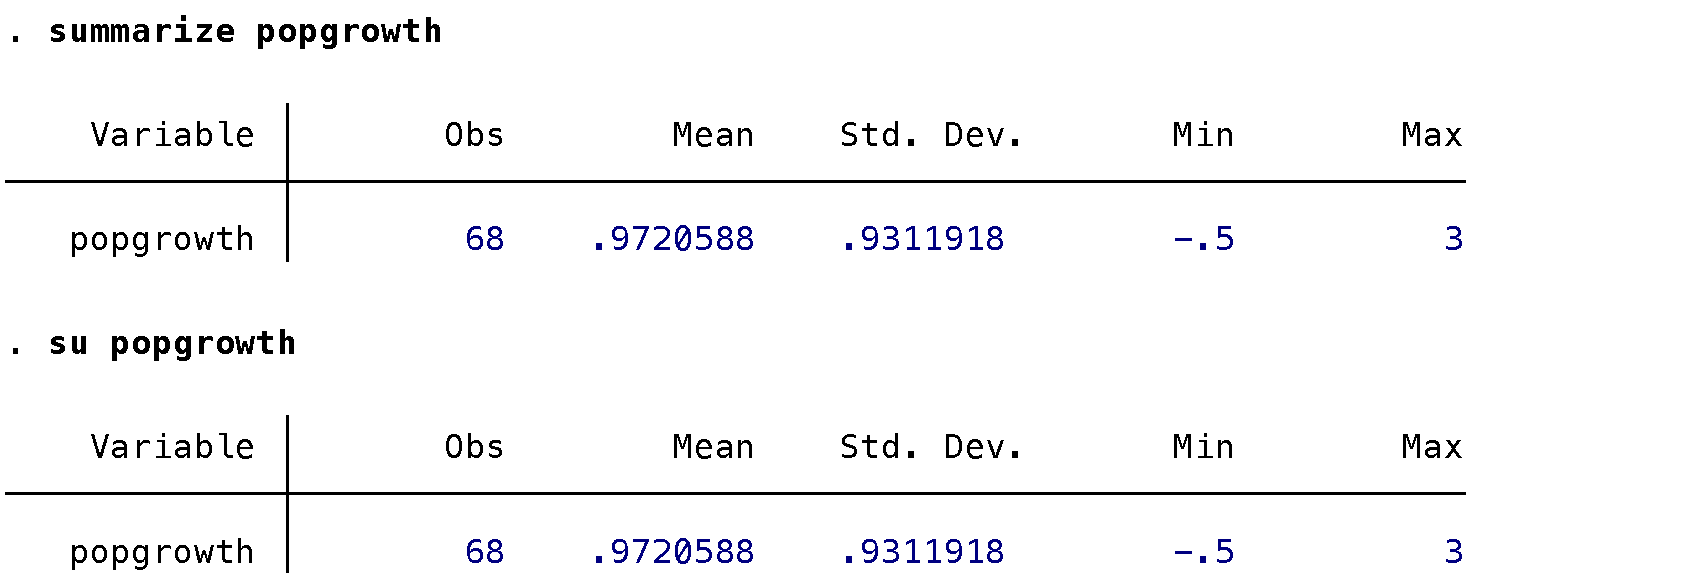
\includegraphics{lifeexp-summarize}\\[1em]

	Abbreviations exist for most commands and come in handy especially with commands such as \cmd[tab]{tabulate}, \cmd[d]{describe} or even \cmd[h]{help}. They also work for options like the \coab{d}{detail}{summarize} option for the \cmd[su]{summarize} command:\\[1em]%
	
		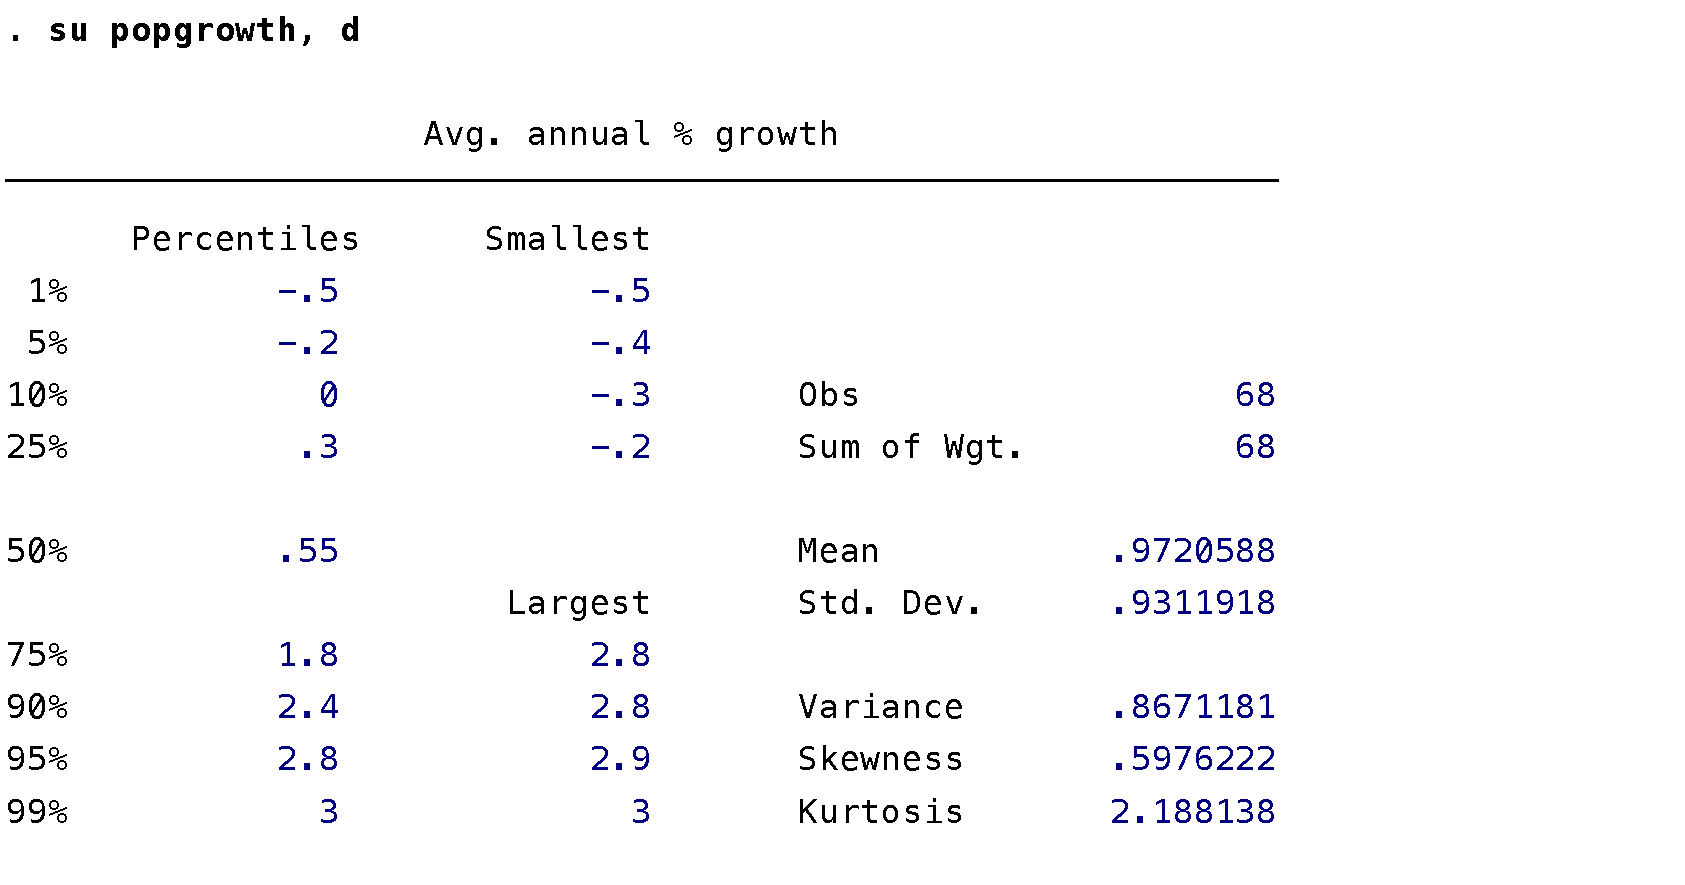
\includegraphics{lifeexp-summarize-d}\\[1em]

	%
	%
	\item[\smallcaps{Installing commands}]%
		\index{Stata!Packages (additional commands)}%
	%
	Stata can install additional commands written by users with programming skills. New commands can be installed by downloading packages from the \SSC server with the \cmd{ssc install} command, which is used at a few points in this guide to install some of these packages. You can install the \cmd{fre} command right away by typing the following command:%
		
	\begin{docspec}
		ssc install fre
	\end{docspec}
		
	Unless you are offline or already have installed the \cmd{fre} package, you should get a few result lines indicating where the package was installed on your hard drive:\\[1em]%
		
	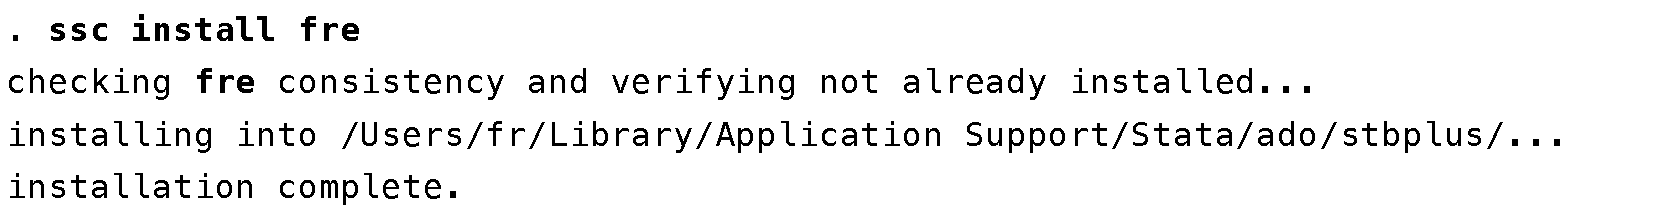
\includegraphics{ssc-install-fre}\\[1em]
		
	Other handy user-contributed commands have been installed as part of the course setup that you ran in the previous section.%
\end{description}

	%
	%
	\subsection{Working from a do-file}%
		\label{sec:do-files}%
		\index{Stata!Do-files}%
	%
	% command execution
	% comments
	% log
	%

	\index{Replication|seealso{Stata!Do-files}}%
	\newthought{When you run Stata commands} to explore a dataset, you are programming `on the fly', typing commands directly into the Stata command line to get quick results. But when you want to structure a complete analysis of your data, you need to record your commands to a script, which is a plain text file containing Stata code. An important part of your work in this course will therefore be to code your analysis into a script.%
	
	Coding your analysis is meant to provide yourself as well as others with the means to replicate your analysis. Maintaining a record of your operations—and commenting them inside as well as outside the code—will not only ensure that others can read and reproduce your work, but also that \emph{you} will be able to remember, in a few months or so, what you precisely ended up doing on your project.%
	
	Making your research fully replicable is not an option in this course: you are required to provide the code for your analysis. Replication also means that you should \hlred{\textbf{keep your original datasets unmodified}}: you will not need to save your modifications because you will instead save the instructions that allow any Stata user with the original data source to prepare it and analyze it as you have.%
	
	The logic of replicability (or reproducibility) outlined here 
	
	\newthought{Stata scripts} end with the \texttt{.do} extension and are called \textbf{do-files}.%
		 \footnote{Stata do-files will usually show as plain text in your Internet browser; if the browser adds a \texttt{.txt} extension to a do-file when downloading it, make sure that you rename the file to \texttt{.do} for Stata to recognize it as a do-file.} %
		%
		It will be one of your main missions throughout the course to learn how to structure and to write such a document. You will be given plenty of examples through a new course do-file every week, and the short vignette that follows will show you some essential aspects of working in Stata from a do-file.%
		%
		%
		
		\begin{marginfigure}
			
\includegraphics[width=.75\textwidth]{stata-do-icon}
			\caption{Stata~12 do-file icon.}
			\label{fig:stata-do}
		\end{marginfigure}

	\begin{description}
	\item[\smallcaps{Create an empty do-file}] Type \cmd{doedit} in the Command window to open a blank Stata do-file, which is your first piece of draft Stata code. Let's write a few lines into it:%

		\begin{docspec}
		  * François Briatte, first do-file\\[1em]%
			%
		  * Load UN data.\\%
			sysuse lifeexp, clear\\[1em]%
			%
			* Describe the data.\\%
			d\\[1em]%
			%
			* Summarize life expectancy\\%
			su lexp\\[1em]%
			%
			* Scatterplot.\\%
		  sc lexp safewater\\[1em]%
			%
			* ttyl\\
		\end{docspec}

		\emph{Step-by-step explanations:}
		
		\begin{enumerate}
			\index{Stata!Comments (code)}%
			\item First type in your name, preceded by an asterisk and a space. You will notice that the line will turn green, to indicate that it is a \textbf{comment}. Comments are for human readers of the code and are not evaluated by Stata, just passively printed to the Results window.%
			
			\item Now add the \cmd{sysuse} command that asks Stata to load a demo dataset in memory, removing any previous unsaved data. If you have run the previous examples, the same dataset will be loaded again.%
			
			\item Finally, add the \cmd[d]{describe} command to list the variables, the \cmd[su]{summarize} command to inspect the life expectancy variable, and the \cmd[sc]{scatter} command to produce a plot of the relationship between life expectancy and access to safe water.%

		\end{enumerate}

		Stata shows the code of your do-file in monospaced font with line numbers and colored syntax. The do-file editor should look like Figure~\ref{fig:hello-world-draft} on my system, which also highlights the currently selected line:%

		\begin{figure}%
			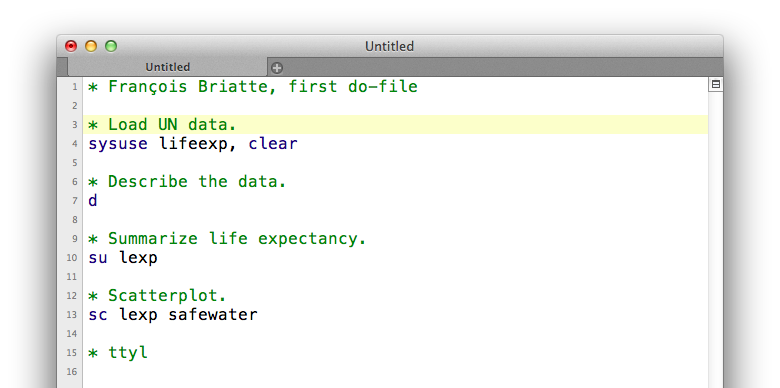
\includegraphics[width=\textwidth]{hello-world-draft}%
			\caption{A draft do-file using the \texttt{lifeexp} dataset.}%
			\label{fig:hello-world-draft}%
		\end{figure}

		\item[\smallcaps{Opening and saving do-files}] Once you are done copying and editing the demo code, save the do-file%
		%
		\footnote{Use \texttt{Cmd-S} (Mac) or \texttt{Ctrl-S} (Win) from your keyboard.} %
		%
		as \texttt{draft.do} in your \code folder, where you should keep all your do-files within the \SRQM folder.%
		
		Now close your first draft and return to the Stata Command window. If you have saved your draft as \texttt{draft.do} into the \code folder, as requested, then Stata will be able to open it with the following command:%

		\begin{docspec}
			doedit code/draft
		\end{docspec}
		
		The \cmd{doedit} command opens do-files from the current working directory, which should be the \SRQM folder for the duration of the course. You can open the course do-files by listing them in the \code folder, using a similar command to the one used previously with datasets:%
		
		
		 and then opening them with \cmd{doedit}.%
		
		
		\hlred{\textbf{{Note:} opening a do-file by double-clicking it is not recommended}, because Stata will quietly change the working directory to the location of the do-file.} The exact same problem exists with datasets. In both cases, you will have to set the working directory back to being the \SRQM folder.%

		Click anywhere on line 2 of your draft do-file and then press \texttt{Cmd-L} (Mac) or \texttt{Ctrl-L} (Win) to select it in full. Then, press \texttt{Shift+DownArrow} or \texttt{Shift+UpArrow} to select the line below or above it. Finally, press \texttt{Cmd-A} (Mac) or \texttt{Ctrl-A} (Win) to select all three lines.%
 
 		\item[\smallcaps{Running do-files}]

		To execute a do-file, press \texttt{Cmd-Shift-D} (Mac) or \texttt{Ctrl-D} (Win). The first line is a comment, as indicated by the asterisk at the beginning of the line, so executing it will not accomplish anything: Stata will just print it to the Results window.%
  
The second and third lines of your do-file will be printed to the Results window with their respective results. The \cmd{cd} command should print the path to your \SRQM folder, and the \cmd{di} command will print a `hello' message, as shown in Figure~\ref{fig:hello-world-result}.
  
\begin{figure}%
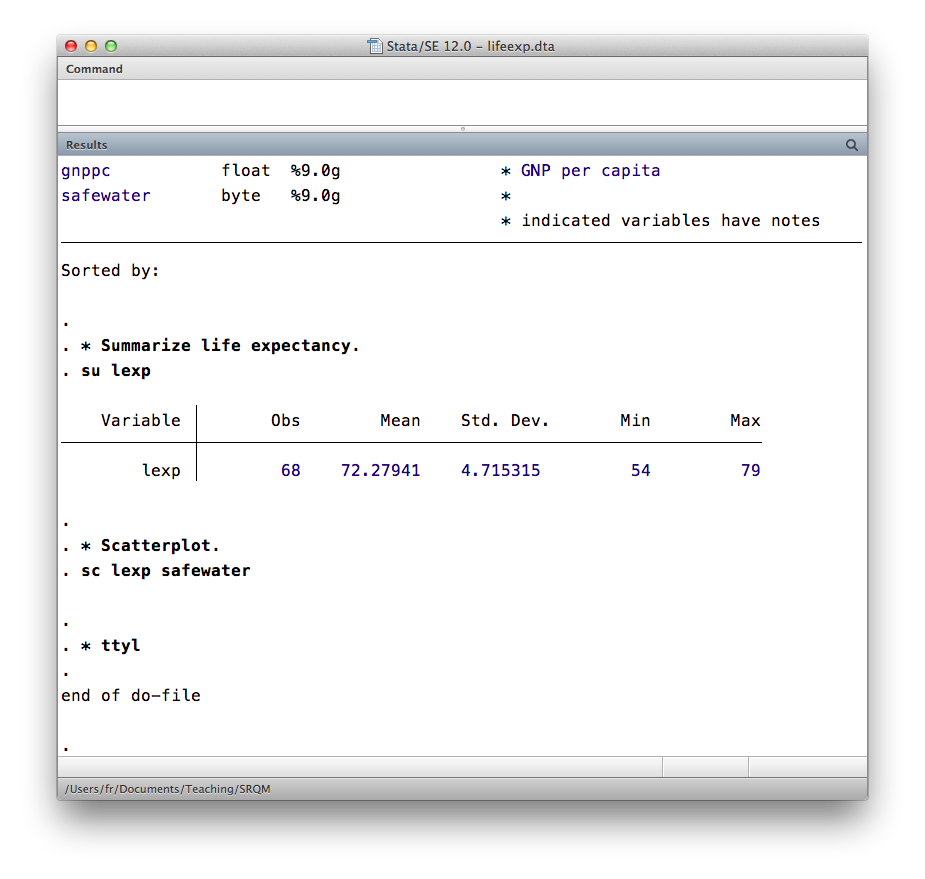
\includegraphics[width=\textwidth]{hello-world-result}
\caption{`Hello World' in Stata.}
\label{fig:hello-world-result}
\end{figure}

\hlred{\textbf{Important:} check your commands for typos and syntax errors.} If your code fails to execute, Stata will send some red ink to the Results window. Check the code against the correct syntax, looking for forgotten (or extra) letters or spaces.
  
\hlred{\textbf{Important:} be careful with copy-pasting to the Command window.} Copy-pasted commands that contain line breaks (\cmd{///}), for example, will not work properly. This point is covered again in the first course do-file.

% \item[Keyboard shortcuts]
  
You can switch between windows from the keyboard: use \texttt{Cmd-`} (Mac) or \texttt{Alt-Tab}. Have a look at the keyboard shortcuts in the `Window' command to learn similar tricks: for example, on Mac~OS~X, \texttt{Cmd-1} switches to the Command window.
  
%%% -- old : replication

The log is a text file that, once open with log using, will save every single command you enter in Stata as well as its results. Systematically logging your work is good prac-tice, even when you are just trying out a few things. Logs can be closed with the log close command followed by the name of your log if it has one:


Comments will also be saved to the log file, which is particularly useful when you have to read through your work again or share it with someone. In the example above, all comments, commands and results were saved to the log file.
% % %

Finally, open the first course do-file, which is your homework for the first week of class:

\begin{docspec}
doedit replication/week1
\end{docspec}

Follow the comments in this do-file to revise this section, learn a few more commands and briefly explore the course datasets.

%% -- old :: LOGS

Logs are useful to save every operation and result from a practice session. If you need someone else to replicate your work, however, you just need to share the commands you entered, along with the comments that you wrote to document your analysis. Files that contain commands and comments are called do-files.
Writing do-files is a crucial aspect of this course. Absent of a do-file, your work will be mostly incomprehensible, or at least impossible to reproduce, to others. Your do-file should include your comments, and it should run smoothly, without returning any er-rors. You will discover that these steps require a lot of work, so start to program early. To open a new do-file, use either the doedit command or the ‘File > New Do-file’ menu (keyboard shortcut: Ctrl-N on Windows, Cmmd-N on Macintosh).
You should take inspiration from the do-files produced for the course to write up your own do-file for your research project. All our do-files are available from the course web-site. This course requires only basic programming skills, as illustrated by the do-files that we run during our practice sessions. More sophisticated examples can be found online.
To execute (or ‘run’) a do-file, open it, select any number of lines, and press Ctrl-D in Stata for Windows or Cmmd-Shift-D in Stata for Macintosh. You can also use either the GUI icons on the top-right of the Do-file Editor window, or use the do or run com-mands. Use the Ctrl-L (Windows) or Cmmd-L (Macintosh) keyboard shortcuts to select the entire current line in order to run it.
Get some practice with do-files as soon as possible, since your coursework will include replicating one do-file a week. Replicating is nothing more than reading through the comments of a do-file, while running all its commands sequentially.

\end{description}
%
%
% 1.3 course setup
%
%
% 1.2
%
\section{Coursework}%

\newthought{The approach to social science} that we follow in this course is driven by a dual logic of inquiry: we start with the description of quantitative data, and we end with its analysis through statistical models. The procedures involved in this process are computational and require some technical knowledge of computers and mathematics.%
	%
	%

	%%% They’re someone who can ask and answer questions about and with data.
	%%% http://www.analyticstory.com/hadley-wickham/

	%%% I A key principle in applied statistics is that you should be able to connect between the raw data, your model, your methods, and your conclusions

	%%%%Controlled experiments are the gold standard, but I never do them!

%%% I (Some) computer scientists' view: we don't need controlled experiments; we can automatically learn from observational data

%%% I Psychologists' view: each causal question requires its own experiment

%%% I Observational scientist's version: each causal question requires its own data analysis

%%% Sample surveys (for the problem of extending from sample to population)

%%% Descriptive observational research (for the problem of modeling complex interactions and response surfaces)

%%%Political science is largely an empirical discipline. That is, most of us studying politics do so because we are motivated by real world political events, either historical, current, or even events yet to happen. We want to know why these events happen and how to make sense of them. Political science trys to answer these questions in a rigorous way. Data analysis is thus a critical component of political science, serving two important purposes: (1) providing numerical descriptions or summaries of political phenomena, facilitating comparisons across time, countries, states, people, etc; (2) testing theories, models and hypothesis about politics.


% All this is to say that this class involves a little math. Or, as I like to put it, this class is ‘‘techie for fuzzies’’: an introduction to the way political scientists use the tools of statistics to rigorously understand political events. I assume virtually zero mathematical background on your part, either because you didn’t take math in high school or because you’ve forgotten it. I assume no prior background with using computers for data analysis. The classes will have a heavy ‘‘show-and-tell’’ feel to them, where I will use statistical software to do data analysis.

%%%forecast the effects of interventions, the trajectory of existing trends, and the likely strategies

%%% http://understandingsociety.blogspot.fr/2009/01/predictions.html

% 1.2.1
%
\subsection{Course outline}%
  \index{Course!Outline and readings}
	%
	%

\newthought{This course} follows the standard regulations of Sciences Po, \ie, attendance is compulsory, every class comes with homework and readings, and plagiarism on any element of coursework is strongly sanctioned. Please turn to your academic regulations for more details on any of these topics.%

The course itself is organised in twelve two-hour sessions that run over a single semester. Its content is structured around three teaching goals:%

\begin{enumerate}
  
  % 1. Statistics

	\label{sec:textbooks}%
	\index{Course!Readings}%
  \item The course covers some \textbf{essential aspects of statistical analysis}, from describing variables to running regression models.%
  
  This learning objective requires that you read from textbooks that apply fundamental statistical theory to social science research. The primary textbook for this course is \citetitle{Urdan:2010a}\footcite{Urdan:2010a}, one of the shortest and most effective introduction to the course topics. %
	
	Towards the end of the class, we turn to \citetitle{FeinsteinThomas:2002d}\footcite{FeinsteinThomas:2002d}, a clearly worded introduction to quantitative methods for qualitatively-minded social scientists, for additional clarifications on regression modelling.%
  
	\index{Course!Syllabus}%
  Both textbooks appear in the course syllabus%
		\footnote{\url{https://github.com/briatte/srqm/blob/master/course/syllabus.pdf?raw=true}} %
    as well as in the final bibliography of this document. Please read the course syllabus in full at that stage, and copy the reading schedule to your agenda.%
		
  The textbook readings for this course will give you a more detailed view of statistics than this guide can provide. Furthermore, since the course slides are mostly trivia taken from the course blog,%
  \footnote{\url{http://srqm.tumblr.com/}} %
    you really have no other choice than to take the time to go through the assigned readings. The weekly readings appear at the beginning of each section of this guide, in the course syllabus, and on the course website.%

  % 2. Stata

  \item The course also explains \textbf{how to operate Stata} for basic data analysis and visualization.%

    \newthought{There will be one Stata do-file to study per week of class.} We will start looking at the do-file in class, and you will be asked to finish replicating it at home. Some online tutorials and Stata Press handbooks, like the recent one by \citeauthor{Mitchell:2012a} on applied regression,\footcite{Mitchell:2012a} can also be used as additional companions.%
		\footnote{See an indicative list of tutorials and books on the course website and on the course wiki: \url{https://github.com/briatte/srqm/wiki/stata}} %
    
    The do-file for the first week covers basic Stata settings and data exploration commands. It will show you how to start exploring the course datasets. Your weekly mission is to replicate the do-file of the current session. After running through the setup described in Section~\ref{sec:course-setup}, the following command will open the do-file for Week~1:%

      \begin{docspec}
        doedit code/week1.do
      \end{docspec}

     \newthought{Read through the do-file and execute (run) its commands sequentially}, reading the comments that precede each block of code. This practice (replicating the course do-files) will show you how to code various things in Stata, which will become handy when you start writing code for your own research project.%
    
     The baseline advice to survive the computing component of the course is very simple: practice by reading and writing code every week of class. If this is going to be the only time in your student life where you get to write statistical code, make sure that you get the most out of it. There is a fair chance that you will be offered to use that skill one day.%
  %

  % 3. Research

  \index{Course!Research projects!Final paper}%
  \item The course finally works assists students to work in pairs over \textbf{small-scale research projects}, on which the grading for the course is based.%
  
    Each student pair submits two draft versions of their empirical analysis (Stata code) and analytical report (research paper) during the semester, and one final version of their at the end of the class. The steps that each student pair needs to take throughout the semester to complete their research projects can be summarised as follows:%

    \begin{itemize}
      \item \textbf{setting up your computer} to follow the course and access the teaching material from the \SRQM folder (Weeks~1--2; Section~\ref{ch:intro});%
      \item \textbf{registering a research topic} with a student partner from your class in the course projects list (Weeks~2--3);%
      \item \textbf{exploring the course datasets} to find variables related to your research topic and select some variables of interest (Weeks~3--4; Section~\ref{ch:data});%
      \item \textbf{submitting your first draft} that presents the topic, the data the distributions of the variables under scrutiny (Weeks~4--5; Section~\ref{ch:distr});%
      \item \textbf{revising your draft} and resubmitting it with additional significance tests of associations in the data (Weeks~5--8; Sections~\ref{ch:asso} and \ref{ch:ols}); and%
      \item \textbf{submitting your final paper} in which you model your data with linear or logistic regression (Weeks~9--12; Sections~\ref{ch:lin} and \ref{ch:log}).%
    \end{itemize}

    \newthought{The deadline} for the first draft is generally set to mid-term (Week~5). The deadline for the revised draft is generally set to Week~10. The deadline for the final paper is generally set to the last course session. In order to make all groups benefit from the challenges that arise in each project, you will be offered to submit questions to collective FAQs before every deadline.%
    %

    \hlred{Exact deadlines and all other project instructions are covered exclusively in class, which is why you should \textbf{attend every week and catch up if absent}.} The course sessions are cumulative: you cannot just skip one as if it had never happened. Your stress and workload \emph{will} increase if you skip a week with the hope of catching up later, and you will \emph{not} be able to fix your project if you let it rest.%
    %

		\newthought{Please read} \citeauthor{White:2005a}'s \citetitle{White:2005a}%
      \footcite{White:2005a} %
      for a refresher on how to write an empirical research paper. If you have never carried empirical research before, please also turn to \citeauthor{BoothWilliams:2003v}'s \citetitle{BoothWilliams:2003v}%
      \footcite{BoothWilliams:2003v} %
      for a detailed explanation on how to prepare a research project. All other teaching material for the research projects paper templates and example papers, is distributed through Google Drive in class.%
    % ^^^^^^^ 
    % replace by internal Google Documents support at Sciences Po (2013)?

		You are encouraged to use your research paper for other purposes than this course: think of it as work that you will be able to add to your student portfolio. Some students have used the coursework from this class to draft \textsc{Msc} dissertations, working papers or essays from other classes on research design and research methodology. Other students have used Stata for other projects in organizations that either consume or produce data.%
      \footnote{Examples from past years include a lot of consulting work on urban areas, research on land law and its effects on economic development, and estimating the number of refugees in a given geographical area to help plan the work of a nongovernmental organization.}%
		%
    
\end{enumerate}

% 1.2.2
%
\subsection{Course setup}%
	%
	%
	\label{sec:course-setup}%
	\index{Course!Setup}%
	%
	%

	\newthought{This section} explains how to set up Stata to follow the course. It assumes very little knowledge of computers or Stata, but please make sure that you have read through the previous section first. \hlred{\textbf{Make sure that you successfully set up your computer} for the course, and that you know how to run the setup again if needed.}%

	The setup below has been tested on Sciences Po workstations equipped with Stata~11. You might run into issues with this setup only if you use a computer with heavy user restrictions or with a really old copy of Stata. Please let us know if the setup fails.%
    \footnote{GitHub users can report issues on the course repository: \url{https://github.com/briatte/srqm/issues}}%
	
	% i
	%
	\paragraph{Get the teaching material}%
		\label{sec:teaching-pack}%
		\index{Course!Teaching material}

	\newthought{The `Teaching Pack' for this course comes in a single folder,} called the \SRQM folder, which you will have to access very frequently inside and outside class. Download and unzip the folder from its webpage%
		\footnote{\url{http://f.briatte.org/srqm/}} %
		or use the copy provided in class, and keep the \ZIP archive of the folder as a backup.%
		
	\hlred{Move the \SRQM folder to a \textbf{stable location} that you can easily locate on your hard drive, and keep it at that same location throughout the entire course.} Most users deal with this requirement by putting the \SRQM folder with the rest of their study files and then creating an alias to it on their Desktop.%
	
	Use any method that does not involve clicking for two full minutes to access the \SRQM folder, and do not rename its enclosing folders. For simplicity, leave the folder name to \SRQM for the class, and rename it to whatever you like at the end of the semester.%
	
	At that stage, \textbf{check the contents} of the \SRQM folder. The \SRQM folder contains the entire course material, minus the copyrighted textbooks and Stata software. The full contents of that folder, shown in Figure~\ref{fig:srqm-folder}, must stay available on your hard drive during the entire course.%
		%
		%

		\begin{figure}%
		  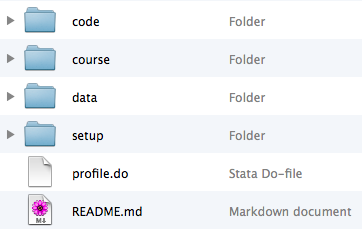
\includegraphics[width=\textwidth]{srqm-folder}
      
		  \caption{The contents of the \SRQM folder should match %
			this screenshot from a \OSX setup.}
		    \label{fig:srqm-folder}
		\end{figure}
		%
		%
		
	The \course folder contains the course slides and syllabus, as well as this guide. The \data folder contains a selection teaching datasets, and the \code folder will host the course do-files (covered below at p.~\pageref{sec:do-files}). The \setup folder and \filename{profile.do} files provide additional course functionalities. All folders are required for the course to roll out properly.%
		%
		%	\index{Computers!File and folder paths}%

	\index{Computers!URLs}%
	You need to understand the file structure of the course to understand how Stata will locate its files and folders from their \textbf{paths}. The path to the \SRQM folder, for example, might look like this on \OSX:\\[1em]%
	
	\begin{docspec}
		/Users/fr/Documents/Teaching/SRQM
	\end{docspec}
	
	The beginning of that path is often abbreviated through a tilde, so that \texttt{~/} designates the user folder. Stata understands that `tilde expansion' notation. Stata for Windows also understand paths with \texttt{\textbackslash} backslashes slashes as used in Windows, where the path generally starts on the \texttt{C:} drive:%

	\begin{docspec}
		C:\textbackslash{}Users\textbackslash{}Ivo\textbackslash{}Desktop\textbackslash{}SRQM
	\end{docspec}
	
	Once a folder has been set as the \emph{working directory}, Stata can locate files and folders from within it by using relative paths. The example below shows the relative path of the \texttt{nhis9711.dta} dataset in the \texttt{\data} folder:\\[1em]%
	
	\begin{docspec}
		/Users/fr/Documents/Teaching/SRQM/\hlred{\underline{data/nhis9711.dta}}
	\end{docspec}

	File paths are used in Stata to open and save datasets and other types of files. In some cases, it is also possible to open files from online sources by specifying their \URL. A \URL is an Internet address like the one that brings up the course webpage.%
		\footnote{\url{http://f.briatte.org/teaching/quanti/}}%
		%
		%
	
	We will use file paths and \URL\ s extensively throughout the course, so make sure that you understand both. I do my best to keep things tidy on my end by using Internet shortlinks and simple, informative folder and file names for the course material. You will have to do the same on your end.%
		%
		\footnote{For instance, you will be required to submit your work under a specific group name that includes your family names in alphabetical order.}%
		%
		%

	% ii
	%
	\paragraph{Set your working directory}%
		\label{sec:working-directory}%
		\index{Course!Teaching material}

  \newthought{Open Stata.} \OSX users can simply double-click the application icon. \hlred{\textbf{Windows users} will have to run Stata with administrator privileges: do this by right-clicking the Stata application icon then selecting `Run as Administrator.'} This will allow Stata to save files anywhere on the hard drive, which is required only for this setup.%
	 
	You are now going to set the working directory, which is the folder in which Stata opens and saves files by default. From the `File' menu, choose `Change working directory...', then select the \SRQM folder and press \texttt{Enter}. You will see something like the following printed in the Results window, that is, a folder path ending with the \SRQM folder:\\[1em]%
	
		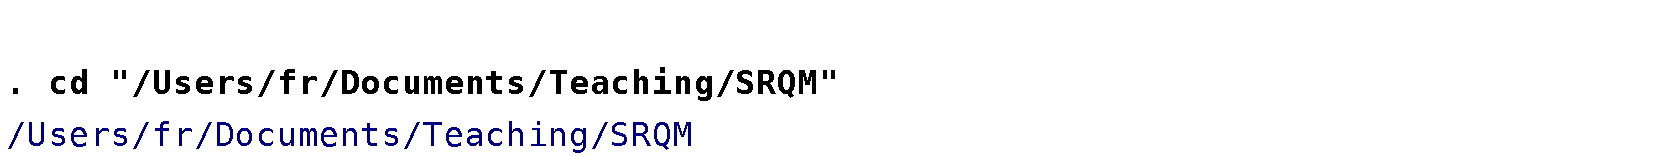
\includegraphics{srqm-cd}\\[1em]

	As the code output shows, the Stata command to do what you did through the `File' menu is \cmd{cd}, for `\underline{c}hoose \underline{d}irectory,' followed by the path to the desired folder. Now that you have learnt a Stata command, try it out by typing the following lines in the Command window and pressing \texttt{Enter} to execute each line:%
	
	\begin{docspec}
		cd ..\\
		cd SRQM
	\end{docspec}
	
	The first command, \texttt{cd ..}, changes the working directory to the enclosing folder, which in my case is the \texttt{Teaching} folder. The second command returns to the \SRQM folder and makes it the working directory again:\\[1em]%
		
	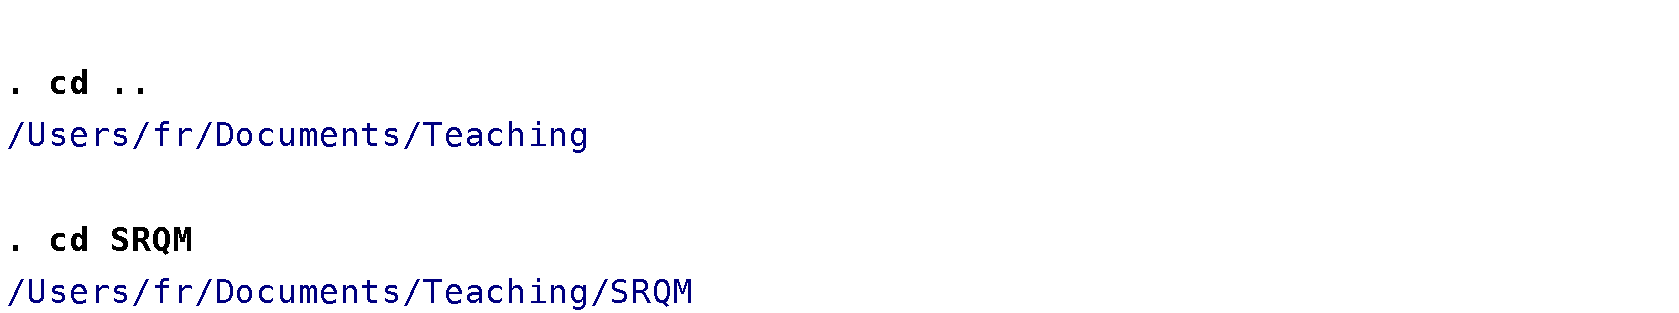
\includegraphics{srqm-cd-back}\\[1em]
	
	You can also list the contents of the working directory with the \cmd{ls} command. The example below will show the full contents of the \SRQM folder with detailed file information:%
	
		\begin{docspec}
			ls
		\end{docspec}

		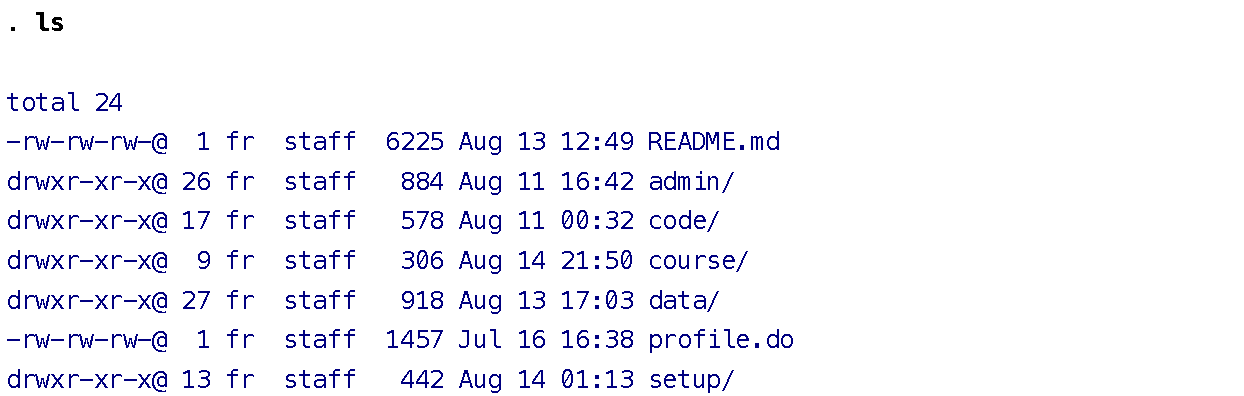
\includegraphics{srqm-ls}\\[1em]
			
	The \cmd{ls} command below will produce a more focused output by listing only the files located in the \data folder that end with the \ext{.dta} extension, which is the Stata dataset format (Figure~\ref{fig:stata-dta-icon}):%

		\begin{marginfigure}
			
\includegraphics[width=.66\textwidth]{stata-dta-icon}
			\caption{Stata~12 dataset icon.}
			\label{fig:stata-dta-icon}
		\end{marginfigure}

		\begin{docspec}
			ls data/*.dta, w
		\end{docspec}
			 
	The command will list the teaching datasets used in the course, showing only their filenames because you passed the \coab{wide}{w}{ls} option to it:\\[1em]%
 
		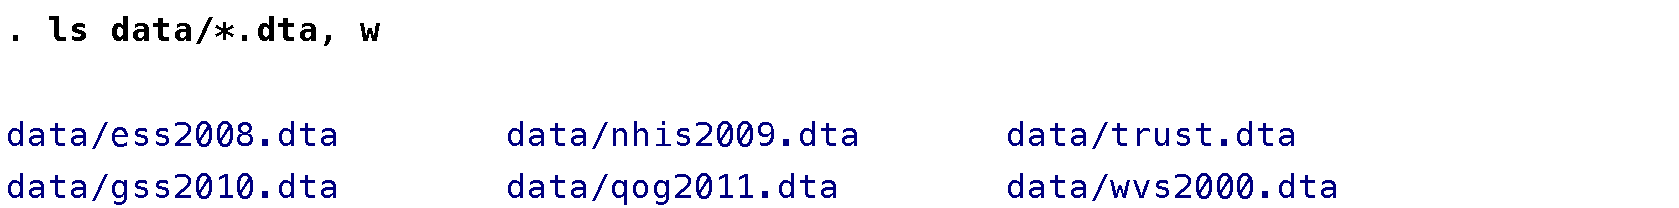
\includegraphics{srqm-ls-dta}\\[1em]
	
	To finish this little exercise with folder navigation from the command line, make sure that your working directory is the \SRQM folder. Use the \cmd{pwd} command to get the path printed once more:%
	
		\begin{docspec}
			pwd
		\end{docspec}
	
	Your working directory should again end with the \SRQM folder, which is what we need to run the course setup in the next section:\\[1em]%
	
		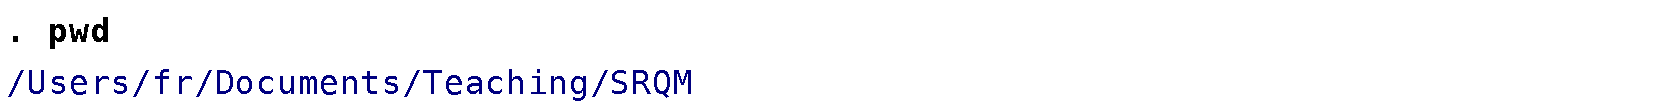
\includegraphics{srqm-pwd}\\[1em]
  
	% iii
  %
  \paragraph{Run the \SRQM setup}%
		\label{sec:setup}%

	To finish setting up your computer for the course, make sure that you are connected to the Internet, then type the following command in the Command window and press \texttt{Enter}:%
		%
		%
		
		\begin{docspec}
			run profile
		\end{docspec}
	
	\hlred{\textbf{Note:} the command will not work if you have not set the \SRQM folder as your working directory}, and that its syntax is a strict one: do not add capital letters, separate the words \texttt{run} and \texttt{profile}, and of course, use the exact spelling.%
	
	This command will trigger a bunch of setup utilities that install the additional Stata commands listed in Table~\ref{tbl:additional-commands}, uncompress the course datasets and adjust some Stata system options.%
		%
		\footnote{For example, the setup adjusts Stata memory on older versions of Stata to deal with some of the larger course datasets. Stata~12 now handles memory automatically.} %
		%
		%
		
	\bigskip

\begin{fullwidth}
	\begin{table}
		\footnotesize
		\begin{tabular}{lll}
		\toprule
		Package & Description \\
		\midrule
		\emph{Installed from the \SSC server:} & & \\
	  \quad \pkg{estout} & export regression results \\
		\quad \pkg{fre} & frequencies with value labels \\
	  \quad \pkg{kountry} & standardised regions and country names\\
	  \quad \pkg{leanout} & simplified regression results\\
		\quad \pkg{lookfor\_all} & search for variables across datasets \\
	  \quad \pkg{mkcorr} & export correlation tables\\
	  \quad \pkg{plotbeta} & regression coefficient plots \\
    % \quad \pkg{qog} & download \QOG data\\
		\quad \pkg{scheme-burd} & graph scheme \\
		\quad \pkg{spineplot} & mosaic plots \\
	  \quad \pkg{spmap} & maps \\
	  \quad \pkg{tab\_chi} & residuals for Chi-squared tests\\
	  \quad \pkg{tabout} & export summary statistics\\
	  \quad \pkg{wbopendata} & download World Bank data\\
		\addlinespace
		\emph{Installed from elsewhere:} & & \\
		\quad \label{install-gstd01}\cmd{gstd01} & standardize a variable to $0$-$1$\\%
    %; used at p.~\pageref{sec:gtsd01} \\
		\quad \label{install-clarify}\pkg{clarify} & simulation\\%
    %; used at p.~\pageref{sec:clarify} \\
    % \quad \pkg{schemes} & graph schemes \\
		\emph{Installed with the course setup:} & & \\
    % \quad \pkg{repl} & replication utility \\
		\quad \cmd{srqm} & course utilities \\
    \quad \cmd{sbar} & plots for categorical data\\
		\quad \cmd{stab} & export summary statistics tables \\
		\bottomrule%\\[1em]
		\end{tabular}
		%
		\caption{Additional commands installed by the course setup.}
		\label{tbl:additional-commands}
	\end{table}
\end{fullwidth}

%
  
	You will get a `\texttt{Hello!}' message when the setup is complete.%
	
  \hlred{\textbf{Note:} if you move or rename the \SRQM folder, the setup will break and you will have to repeat the steps covered in the previous paragraphs to fix the issue:}%
		%
		%	
		\begin{enumerate}
			\item run as administrator (if using Windows),
			\item select the \SRQM folder as the working directory, and
			\item type \texttt{run profile} to go through setup again.
		\end{enumerate}
	  
	The setup overwrites the \filename{profile.do} file of the Stata application folder to redirect it to the \SRQM folder for the time of the course. From there, it runs another \filename{profile.do} file that verifies the integrity of the teaching material and reruns parts of the setup if necessary.%
		%
		%
		
	The setup also loads the \cmd{srqm} teaching utilities, like \cmd{srqm\_get}, which is used in class to download the latest version of the course material from a temporary course server, and \cmd{stab}, which is used to produce \underline{s}imple \underline{tab}les of summary statistics (see its detailed instructions at p.~\pageref{cmd:stab}).%
    %
    %
		
  \newthought{At the end of the course}, delete the \texttt{profile.do} from the Stata application folder to stop automatically setting the \SRQM folder as your working directory. Alternately, run the \texttt{srqm\_link, clean} command to do so and get a `\texttt{Bye}' message. This will let you work with Stata from any other working directory.%
		%
		%

%
%
\subsection{Course datasets}
	\label{sec:data-sources}
	\index{Datasets!Data sources}%
	%
	%

  \newthought{Stata can load example data} with the \cmd{sysuse} and \cmd{webuse} commands, as shown with the \code{lifeexp} dataset at p.~\pageref{lifeexp}. The course provides its own teaching datasets, listed in Table~\ref{tbl:data-sources}. The course setup will also download two files to plot world maps in Stata.%

  \bigskip
\begin{table}
  \begin{center}
  \footnotesize
  \begin{tabular}{lll}
    \toprule
    Filename & Data & Year(s) \\
    \midrule
    \quad \texttt{ess2008}  & \ess  & Round~4, 2008\\
    \quad \texttt{gss0012}  & \gss  & 2000-2012\\
    \quad \texttt{nhis2009} & \nhis & 2000-2009\\
    \quad \texttt{qog2013}  & \qog  & 2009 ± 3 years\\
    \quad \texttt{wvs2000}  & \wvs  & Wave~4, 2000\\
    \bottomrule
  \end{tabular}
  \end{center}
  \label{tbl:data-sources}%
\end{table}


	All course datasets are in the \data folder, from where they can be loaded into memory with the \cmd{use} command. The command requires that you pass the exact file path of the dataset, and that you include quotes if the file path contains spaces. Note that the \cmd{use} command can also copy data from a \URL, which we might quickly review later on.%

  The example below will load a course dataset in memory:%

		\begin{docspec}
			* Load the National Health Interview Survey, years 2000-2009.\\
			use data/nhis9711, clear
		\end{docspec}

  Stata looks for \ext{.dta} files by default, so the file extension can be omitted from the command. The \opt{clear}{use} option ensures that Stata will load the data even if there is already modified data in memory. Because you are never going to overwrite the original datasets, you are never going to lose anything crucial by doing so.%

	Stata can only open one dataset at the time and opens data silently: if the operation succeeds, nothing is printed on screen, except for a short message if the dataset has been labelled by its creator. All datasets for this course are slightly modified versions of the original ones and will print a short message when opened:\\[1em]%
		
		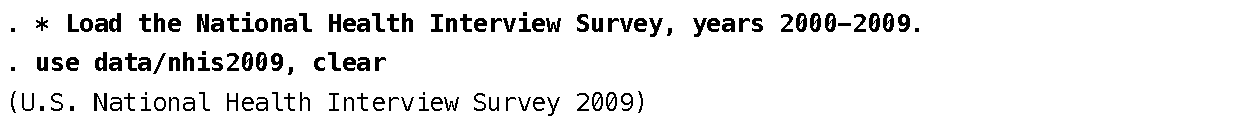
\includegraphics{use-nhis}\\[1em]%

  \newthought{The next paragraphs describe the course datasets}. These are provided in Stata 9/10 \ext{.dta} format on an ``as-is'' basis: please reference their original sources and use them for teaching purposes only. Modifications to the original files are coded in the \texttt{srqm\_data.ado} script, which is part of the course utilities.%
    \footnote{\url{https://github.com/briatte/srqm/wiki/course-utilities}}%
    
  The documentation below shows how to load the datasets in memory from the \SRQM folder with the \cmd{use} command, sometimes with an additional \cmd{if} argument to restrict the data to a particular survey year or round. Further illustrations of how to select a particular segment of your data for analysis are provided in the next sections. You will have to make your own data selection for your research project.%

\paragraph{\ess (\texttt{ess0810})}

The \texttt{ess0810} dataset holds Rounds~4~(2008) and 5~(2010) of the \ess (\ESS).%
	\footnote{\url{http://ess.nsd.uib.no/ess/round4/}}

\begin{quote}
	The \ess (the \ESS) is an academically-driven social survey designed to chart and explain the interaction between Europe's changing institutions and the attitudes, beliefs and behaviour patterns of its diverse populations.%
	\footnote{\url{http://www.europeansocialsurvey.org}}
\end{quote}

Example usage:

\begin{docspec}
  * Load the ESS dataset.\\%
  use data/ess0810, clear\\[1em]%
  %
  * Load latest survey round.\\%
	use data/ess0810 if essround == 4, clear\\[1em]%
  %
  * Load data for one country.\\%
  use data/ess0810 if cntry == "RU"\\[1em]%
  %
  * Load data for two countries.\\%
	use data/ess0810 if inlist(cntry, "CZ", "SK"), clear
\end{docspec}

The \ESS dataset should be used with the following survey weights:

\begin{docspec}
  * Set survey design weights.\\%
	svyset [pw = dweight]
\end{docspec}

See the \ESS weighting guide for details on using additional population weights to use a sample that representative of the European population.%
  \footnote{\url{http://ess.nsd.uib.no/ess/doc/weighting.pdf}} %
  You might also want to take a look at Matthias Ganniger's training module on weigthing the \ESS, which is an excellent five-chapter introduction to the topic.%
  \footnote{\url{http://essedunet.nsd.uib.no/cms/topics/weight/}}

The datasets for both rounds were downloaded from the ESS data server,%
  \footnote{\url{http://nesstar.ess.nsd.uib.no/}} %
  and the codebooks were downloaded from the \ESS data website, on which you can also find a very useful series of booklets that present overall and `topline' results.%
  \footnote{\url{http://ess.nsd.uib.no/}} %
  Check the cumulative dataset for other ESS survey waves,%
  \footnote{\url{http://ess.nsd.uib.no/downloadwizard/}} %
  and refer to the original datasets for nation-specific variables (\eg mother's education in Slovakia or party membership in Belgium).

\paragraph{\gss (\texttt{gss0012})}

The \texttt{gss0012} dataset holds data from the U.S. \gss (\GSS) for years 2000-2012.

\begin{quote}
	The \GSS contains a standard `core' of demographic, behavioral, and attitudinal questions, plus topics of special interest. Many of the core questions have remained unchanged since 1972 to facilitate time-trend studies as well as replication of earlier findings.%
	\footnote{\url{http://www3.norc.org/GSS+Website/}}
\end{quote}

Example usage:

\begin{docspec}
  * Load GSS dataset.\\%
  use data/gss0012, clear\\[1em]%
  %
  * Load latest survey year.\\%
	use data/gss0012 if year == 2012, clear
\end{docspec}

The \GSS dataset should be used with the following survey weights:

\begin{docspec}
  * Set survey design weights.\\%
	svyset vpsu [pw = wtssall], strata(vstrat)
\end{docspec}

% link to Pedlow requires fix
% http://tex.stackexchange.com/questions/12230/getting-percent-sign-into-an-url-in-a-footnote#12233

See Appendix~A of the \GSS codebook%
   \footnote{\url{http://publicdata.norc.org:41000/gss/documents//BOOK/GSS_Codebook_AppendixA.pdf}} %
   and the online technical paper ``Calculating Design-Corrected Standard Errors for the General Social Survey, 1988-2010''%
  \footnote{\url{http://publicdata.norc.org:41000/gss/documents//OTHR/GSS\%20design\%20variables.pdf}} %
   by Steven Pedlow for details, especially if you plan to use older survey years for which the sampling and weighting design are different.%

The data are extracted from the \GSS 1972-2012 cumulative cross-sectional dataset (Release 2, June 2013).%
  \footnote{\url{http://www3.norc.org/GSS+Website/Download/STATA+v8.0+Format/}}

\paragraph{\nhis (\texttt{nhis9711})}

The \texttt{nhis9711} dataset holds sample adult data for years 1997--2011 of the U.S. \nhis (\NHIS).

\begin{quote}
	The \nhis (\NHIS) has monitored the health of the nation since 1957. \NHIS data on a broad range of health topics are collected through personal household interviews. For over 50 years, the U.S. Census Bureau has been the data collection agent for the \NHIS. Survey results have been instrumental in providing data to track health status, health care access, and progress toward achieving national health objectives.%
	\footnote{\url{http://www.cdc.gov/nchs/nhis.htm}} 
\end{quote}

Example usage:

\begin{docspec}
  * Load NHIS dataset.\\%
  use data/nhis9711, clear\\[1em]%
  %
  * Load latest survey year.\\%
	use data/nhis9711 if year == 2011, clear
\end{docspec}

The \NHIS dataset should be used with the following survey weights:

\begin{docspec}
    * Set survey design weights\\
    svyset psu [pw = perweight], strata(strata)
\end{docspec}

See the IHIS/NHIS user notes on variance estimation for more details.%
  \footnote{\url{http://www.ihis.us/ihis/userNotes_variance.shtml}}

The data come from the Integrated Health Interview Series website.%
  \footnote{\url{http://www.ihis.us/}} %
  In the course, we use this dataset to illustrate normality in the distribution of the Body Mass Index in American adults. Our class estimates will slightly differ from the official figures because we will be using the public \nhis files, in which extreme observations of height and weight have been redacted. The data contain an additional variable for race and ethnicity, based on a simplified version of the official classification standard.%
  \footnote{\url{http://www.whitehouse.gov/omb/fedreg_race-ethnicity}}%

\paragraph{\qog (\texttt{qog2013})}

The \texttt{qog2013} dataset holds the \qog (\QOG) Standard cross-sectional dataset in its most recent revision of May~15, 2013. The data are country-level aggregates centered around 2009 $\pm$ 3 years.%

\begin{quote}
	Our research addresses the questions of how to create and maintain high quality government institutions and how the quality of such institutions influences public policy in a broader sense.%
  \footnote{\url{http://www.qog.pol.gu.se/}}%
\end{quote}

Example usage:

\begin{docspec}
  * Load QOG dataset.\\%
  use data/qog2013, clear%
\end{docspec}

The data and codebook come from the \QOG Standard download page.%
   \footnote{\url{http://www.qog.pol.gu.se/data/qogstandarddataset/}}

\paragraph{\wvs (\texttt{wvs2000})}

The \texttt{wvs2000} dataset holds data from Wave~4 (1999-2004) of the \wvs (\WVS).

\begin{quote}
	The \wvs (\WVS) is a worldwide network of social scientists studying changing values and their impact on social and political life. The \WVS in collaboration with EVS (European Values Study) carried out representative national surveys in 97 societies containing almost 90 percent of the world's population. These surveys show pervasive changes in what people want out of life and what they believe. In order to monitor these changes, the EVS/WVS has executed five waves of surveys, from 1981 to 2007.%
	\footnote{\url{http://www.worldvaluessurvey.org/}}
\end{quote}

Example usage:

\begin{docspec}
  * Load WVS dataset.\\%
  use data/wvs2000, clear\\[1em]%
  %
  * Load data for one country (using numeric code).\\%
	use data/wvs2000 if v2 == 4, clear\\[1em]%
  %
  * Load data for two countries (using names).\\%
  use data/wvs2000, clear\\%
  decode v2, gen(country)\\%
  keep if inlist(country, "Iran", "Iraq")\\%
  drop v2%
\end{docspec}

The \WVS dataset should be used with the following survey weights:

\begin{docspec}
  * Set survey design weights.
	svyset [pw = s017]
\end{docspec}

See the \WVS weighting guide for details.%
  \footnote{\url{http://www.jdsurvey.net/jds/jdsurveyActualidad.jsp?Idioma=I&SeccionTexto=0405}}

The data come from the official file found at the \WVS website.%
   \footnote{\url{http://www.wvsevsdb.com/}} %
   This version has encoding issues that are used as examples to teach recoding. The cumulative dataset has different variable names and proper variable encoding. More recent data is also currently getting assembled in Wave~6 (2010-2013) of the \wvs.%
  \footnote{\url{http://www.wvs-online.com/}}
%
%

\stopcontents[chapters]

%
% have a nice day
%
